
% Default to the notebook output style

    


% Inherit from the specified cell style.




    
\documentclass[11pt]{article}

    
    
    \usepackage[T1]{fontenc}
    % Nicer default font (+ math font) than Computer Modern for most use cases
    \usepackage{mathpazo}

    % Basic figure setup, for now with no caption control since it's done
    % automatically by Pandoc (which extracts ![](path) syntax from Markdown).
    \usepackage{graphicx}
    % We will generate all images so they have a width \maxwidth. This means
    % that they will get their normal width if they fit onto the page, but
    % are scaled down if they would overflow the margins.
    \makeatletter
    \def\maxwidth{\ifdim\Gin@nat@width>\linewidth\linewidth
    \else\Gin@nat@width\fi}
    \makeatother
    \let\Oldincludegraphics\includegraphics
    % Set max figure width to be 80% of text width, for now hardcoded.
    \renewcommand{\includegraphics}[1]{\Oldincludegraphics[width=.8\maxwidth]{#1}}
    % Ensure that by default, figures have no caption (until we provide a
    % proper Figure object with a Caption API and a way to capture that
    % in the conversion process - todo).
    \usepackage{caption}
    \DeclareCaptionLabelFormat{nolabel}{}
    \captionsetup{labelformat=nolabel}

    \usepackage{adjustbox} % Used to constrain images to a maximum size 
    \usepackage{xcolor} % Allow colors to be defined
    \usepackage{enumerate} % Needed for markdown enumerations to work
    \usepackage{geometry} % Used to adjust the document margins
    \usepackage{amsmath} % Equations
    \usepackage{amssymb} % Equations
    \usepackage{textcomp} % defines textquotesingle
    % Hack from http://tex.stackexchange.com/a/47451/13684:
    \AtBeginDocument{%
        \def\PYZsq{\textquotesingle}% Upright quotes in Pygmentized code
    }
    \usepackage{upquote} % Upright quotes for verbatim code
    \usepackage{eurosym} % defines \euro
    \usepackage[mathletters]{ucs} % Extended unicode (utf-8) support
    \usepackage[utf8x]{inputenc} % Allow utf-8 characters in the tex document
    \usepackage{fancyvrb} % verbatim replacement that allows latex
    \usepackage{grffile} % extends the file name processing of package graphics 
                         % to support a larger range 
    % The hyperref package gives us a pdf with properly built
    % internal navigation ('pdf bookmarks' for the table of contents,
    % internal cross-reference links, web links for URLs, etc.)
    \usepackage{hyperref}
    \usepackage{longtable} % longtable support required by pandoc >1.10
    \usepackage{booktabs}  % table support for pandoc > 1.12.2
    \usepackage[inline]{enumitem} % IRkernel/repr support (it uses the enumerate* environment)
    \usepackage[normalem]{ulem} % ulem is needed to support strikethroughs (\sout)
                                % normalem makes italics be italics, not underlines
    

    
    
    % Colors for the hyperref package
    \definecolor{urlcolor}{rgb}{0,.145,.698}
    \definecolor{linkcolor}{rgb}{.71,0.21,0.01}
    \definecolor{citecolor}{rgb}{.12,.54,.11}

    % ANSI colors
    \definecolor{ansi-black}{HTML}{3E424D}
    \definecolor{ansi-black-intense}{HTML}{282C36}
    \definecolor{ansi-red}{HTML}{E75C58}
    \definecolor{ansi-red-intense}{HTML}{B22B31}
    \definecolor{ansi-green}{HTML}{00A250}
    \definecolor{ansi-green-intense}{HTML}{007427}
    \definecolor{ansi-yellow}{HTML}{DDB62B}
    \definecolor{ansi-yellow-intense}{HTML}{B27D12}
    \definecolor{ansi-blue}{HTML}{208FFB}
    \definecolor{ansi-blue-intense}{HTML}{0065CA}
    \definecolor{ansi-magenta}{HTML}{D160C4}
    \definecolor{ansi-magenta-intense}{HTML}{A03196}
    \definecolor{ansi-cyan}{HTML}{60C6C8}
    \definecolor{ansi-cyan-intense}{HTML}{258F8F}
    \definecolor{ansi-white}{HTML}{C5C1B4}
    \definecolor{ansi-white-intense}{HTML}{A1A6B2}

    % commands and environments needed by pandoc snippets
    % extracted from the output of `pandoc -s`
    \providecommand{\tightlist}{%
      \setlength{\itemsep}{0pt}\setlength{\parskip}{0pt}}
    \DefineVerbatimEnvironment{Highlighting}{Verbatim}{commandchars=\\\{\}}
    % Add ',fontsize=\small' for more characters per line
    \newenvironment{Shaded}{}{}
    \newcommand{\KeywordTok}[1]{\textcolor[rgb]{0.00,0.44,0.13}{\textbf{{#1}}}}
    \newcommand{\DataTypeTok}[1]{\textcolor[rgb]{0.56,0.13,0.00}{{#1}}}
    \newcommand{\DecValTok}[1]{\textcolor[rgb]{0.25,0.63,0.44}{{#1}}}
    \newcommand{\BaseNTok}[1]{\textcolor[rgb]{0.25,0.63,0.44}{{#1}}}
    \newcommand{\FloatTok}[1]{\textcolor[rgb]{0.25,0.63,0.44}{{#1}}}
    \newcommand{\CharTok}[1]{\textcolor[rgb]{0.25,0.44,0.63}{{#1}}}
    \newcommand{\StringTok}[1]{\textcolor[rgb]{0.25,0.44,0.63}{{#1}}}
    \newcommand{\CommentTok}[1]{\textcolor[rgb]{0.38,0.63,0.69}{\textit{{#1}}}}
    \newcommand{\OtherTok}[1]{\textcolor[rgb]{0.00,0.44,0.13}{{#1}}}
    \newcommand{\AlertTok}[1]{\textcolor[rgb]{1.00,0.00,0.00}{\textbf{{#1}}}}
    \newcommand{\FunctionTok}[1]{\textcolor[rgb]{0.02,0.16,0.49}{{#1}}}
    \newcommand{\RegionMarkerTok}[1]{{#1}}
    \newcommand{\ErrorTok}[1]{\textcolor[rgb]{1.00,0.00,0.00}{\textbf{{#1}}}}
    \newcommand{\NormalTok}[1]{{#1}}
    
    % Additional commands for more recent versions of Pandoc
    \newcommand{\ConstantTok}[1]{\textcolor[rgb]{0.53,0.00,0.00}{{#1}}}
    \newcommand{\SpecialCharTok}[1]{\textcolor[rgb]{0.25,0.44,0.63}{{#1}}}
    \newcommand{\VerbatimStringTok}[1]{\textcolor[rgb]{0.25,0.44,0.63}{{#1}}}
    \newcommand{\SpecialStringTok}[1]{\textcolor[rgb]{0.73,0.40,0.53}{{#1}}}
    \newcommand{\ImportTok}[1]{{#1}}
    \newcommand{\DocumentationTok}[1]{\textcolor[rgb]{0.73,0.13,0.13}{\textit{{#1}}}}
    \newcommand{\AnnotationTok}[1]{\textcolor[rgb]{0.38,0.63,0.69}{\textbf{\textit{{#1}}}}}
    \newcommand{\CommentVarTok}[1]{\textcolor[rgb]{0.38,0.63,0.69}{\textbf{\textit{{#1}}}}}
    \newcommand{\VariableTok}[1]{\textcolor[rgb]{0.10,0.09,0.49}{{#1}}}
    \newcommand{\ControlFlowTok}[1]{\textcolor[rgb]{0.00,0.44,0.13}{\textbf{{#1}}}}
    \newcommand{\OperatorTok}[1]{\textcolor[rgb]{0.40,0.40,0.40}{{#1}}}
    \newcommand{\BuiltInTok}[1]{{#1}}
    \newcommand{\ExtensionTok}[1]{{#1}}
    \newcommand{\PreprocessorTok}[1]{\textcolor[rgb]{0.74,0.48,0.00}{{#1}}}
    \newcommand{\AttributeTok}[1]{\textcolor[rgb]{0.49,0.56,0.16}{{#1}}}
    \newcommand{\InformationTok}[1]{\textcolor[rgb]{0.38,0.63,0.69}{\textbf{\textit{{#1}}}}}
    \newcommand{\WarningTok}[1]{\textcolor[rgb]{0.38,0.63,0.69}{\textbf{\textit{{#1}}}}}
    
    
    % Define a nice break command that doesn't care if a line doesn't already
    % exist.
    \def\br{\hspace*{\fill} \\* }
    % Math Jax compatability definitions
    \def\gt{>}
    \def\lt{<}
    % Document parameters
    \title{Convexity \& concavity tests for single and multivariable functions}
    
    
    

    % Pygments definitions
    
\makeatletter
\def\PY@reset{\let\PY@it=\relax \let\PY@bf=\relax%
    \let\PY@ul=\relax \let\PY@tc=\relax%
    \let\PY@bc=\relax \let\PY@ff=\relax}
\def\PY@tok#1{\csname PY@tok@#1\endcsname}
\def\PY@toks#1+{\ifx\relax#1\empty\else%
    \PY@tok{#1}\expandafter\PY@toks\fi}
\def\PY@do#1{\PY@bc{\PY@tc{\PY@ul{%
    \PY@it{\PY@bf{\PY@ff{#1}}}}}}}
\def\PY#1#2{\PY@reset\PY@toks#1+\relax+\PY@do{#2}}

\expandafter\def\csname PY@tok@w\endcsname{\def\PY@tc##1{\textcolor[rgb]{0.73,0.73,0.73}{##1}}}
\expandafter\def\csname PY@tok@c\endcsname{\let\PY@it=\textit\def\PY@tc##1{\textcolor[rgb]{0.25,0.50,0.50}{##1}}}
\expandafter\def\csname PY@tok@cp\endcsname{\def\PY@tc##1{\textcolor[rgb]{0.74,0.48,0.00}{##1}}}
\expandafter\def\csname PY@tok@k\endcsname{\let\PY@bf=\textbf\def\PY@tc##1{\textcolor[rgb]{0.00,0.50,0.00}{##1}}}
\expandafter\def\csname PY@tok@kp\endcsname{\def\PY@tc##1{\textcolor[rgb]{0.00,0.50,0.00}{##1}}}
\expandafter\def\csname PY@tok@kt\endcsname{\def\PY@tc##1{\textcolor[rgb]{0.69,0.00,0.25}{##1}}}
\expandafter\def\csname PY@tok@o\endcsname{\def\PY@tc##1{\textcolor[rgb]{0.40,0.40,0.40}{##1}}}
\expandafter\def\csname PY@tok@ow\endcsname{\let\PY@bf=\textbf\def\PY@tc##1{\textcolor[rgb]{0.67,0.13,1.00}{##1}}}
\expandafter\def\csname PY@tok@nb\endcsname{\def\PY@tc##1{\textcolor[rgb]{0.00,0.50,0.00}{##1}}}
\expandafter\def\csname PY@tok@nf\endcsname{\def\PY@tc##1{\textcolor[rgb]{0.00,0.00,1.00}{##1}}}
\expandafter\def\csname PY@tok@nc\endcsname{\let\PY@bf=\textbf\def\PY@tc##1{\textcolor[rgb]{0.00,0.00,1.00}{##1}}}
\expandafter\def\csname PY@tok@nn\endcsname{\let\PY@bf=\textbf\def\PY@tc##1{\textcolor[rgb]{0.00,0.00,1.00}{##1}}}
\expandafter\def\csname PY@tok@ne\endcsname{\let\PY@bf=\textbf\def\PY@tc##1{\textcolor[rgb]{0.82,0.25,0.23}{##1}}}
\expandafter\def\csname PY@tok@nv\endcsname{\def\PY@tc##1{\textcolor[rgb]{0.10,0.09,0.49}{##1}}}
\expandafter\def\csname PY@tok@no\endcsname{\def\PY@tc##1{\textcolor[rgb]{0.53,0.00,0.00}{##1}}}
\expandafter\def\csname PY@tok@nl\endcsname{\def\PY@tc##1{\textcolor[rgb]{0.63,0.63,0.00}{##1}}}
\expandafter\def\csname PY@tok@ni\endcsname{\let\PY@bf=\textbf\def\PY@tc##1{\textcolor[rgb]{0.60,0.60,0.60}{##1}}}
\expandafter\def\csname PY@tok@na\endcsname{\def\PY@tc##1{\textcolor[rgb]{0.49,0.56,0.16}{##1}}}
\expandafter\def\csname PY@tok@nt\endcsname{\let\PY@bf=\textbf\def\PY@tc##1{\textcolor[rgb]{0.00,0.50,0.00}{##1}}}
\expandafter\def\csname PY@tok@nd\endcsname{\def\PY@tc##1{\textcolor[rgb]{0.67,0.13,1.00}{##1}}}
\expandafter\def\csname PY@tok@s\endcsname{\def\PY@tc##1{\textcolor[rgb]{0.73,0.13,0.13}{##1}}}
\expandafter\def\csname PY@tok@sd\endcsname{\let\PY@it=\textit\def\PY@tc##1{\textcolor[rgb]{0.73,0.13,0.13}{##1}}}
\expandafter\def\csname PY@tok@si\endcsname{\let\PY@bf=\textbf\def\PY@tc##1{\textcolor[rgb]{0.73,0.40,0.53}{##1}}}
\expandafter\def\csname PY@tok@se\endcsname{\let\PY@bf=\textbf\def\PY@tc##1{\textcolor[rgb]{0.73,0.40,0.13}{##1}}}
\expandafter\def\csname PY@tok@sr\endcsname{\def\PY@tc##1{\textcolor[rgb]{0.73,0.40,0.53}{##1}}}
\expandafter\def\csname PY@tok@ss\endcsname{\def\PY@tc##1{\textcolor[rgb]{0.10,0.09,0.49}{##1}}}
\expandafter\def\csname PY@tok@sx\endcsname{\def\PY@tc##1{\textcolor[rgb]{0.00,0.50,0.00}{##1}}}
\expandafter\def\csname PY@tok@m\endcsname{\def\PY@tc##1{\textcolor[rgb]{0.40,0.40,0.40}{##1}}}
\expandafter\def\csname PY@tok@gh\endcsname{\let\PY@bf=\textbf\def\PY@tc##1{\textcolor[rgb]{0.00,0.00,0.50}{##1}}}
\expandafter\def\csname PY@tok@gu\endcsname{\let\PY@bf=\textbf\def\PY@tc##1{\textcolor[rgb]{0.50,0.00,0.50}{##1}}}
\expandafter\def\csname PY@tok@gd\endcsname{\def\PY@tc##1{\textcolor[rgb]{0.63,0.00,0.00}{##1}}}
\expandafter\def\csname PY@tok@gi\endcsname{\def\PY@tc##1{\textcolor[rgb]{0.00,0.63,0.00}{##1}}}
\expandafter\def\csname PY@tok@gr\endcsname{\def\PY@tc##1{\textcolor[rgb]{1.00,0.00,0.00}{##1}}}
\expandafter\def\csname PY@tok@ge\endcsname{\let\PY@it=\textit}
\expandafter\def\csname PY@tok@gs\endcsname{\let\PY@bf=\textbf}
\expandafter\def\csname PY@tok@gp\endcsname{\let\PY@bf=\textbf\def\PY@tc##1{\textcolor[rgb]{0.00,0.00,0.50}{##1}}}
\expandafter\def\csname PY@tok@go\endcsname{\def\PY@tc##1{\textcolor[rgb]{0.53,0.53,0.53}{##1}}}
\expandafter\def\csname PY@tok@gt\endcsname{\def\PY@tc##1{\textcolor[rgb]{0.00,0.27,0.87}{##1}}}
\expandafter\def\csname PY@tok@err\endcsname{\def\PY@bc##1{\setlength{\fboxsep}{0pt}\fcolorbox[rgb]{1.00,0.00,0.00}{1,1,1}{\strut ##1}}}
\expandafter\def\csname PY@tok@kc\endcsname{\let\PY@bf=\textbf\def\PY@tc##1{\textcolor[rgb]{0.00,0.50,0.00}{##1}}}
\expandafter\def\csname PY@tok@kd\endcsname{\let\PY@bf=\textbf\def\PY@tc##1{\textcolor[rgb]{0.00,0.50,0.00}{##1}}}
\expandafter\def\csname PY@tok@kn\endcsname{\let\PY@bf=\textbf\def\PY@tc##1{\textcolor[rgb]{0.00,0.50,0.00}{##1}}}
\expandafter\def\csname PY@tok@kr\endcsname{\let\PY@bf=\textbf\def\PY@tc##1{\textcolor[rgb]{0.00,0.50,0.00}{##1}}}
\expandafter\def\csname PY@tok@bp\endcsname{\def\PY@tc##1{\textcolor[rgb]{0.00,0.50,0.00}{##1}}}
\expandafter\def\csname PY@tok@fm\endcsname{\def\PY@tc##1{\textcolor[rgb]{0.00,0.00,1.00}{##1}}}
\expandafter\def\csname PY@tok@vc\endcsname{\def\PY@tc##1{\textcolor[rgb]{0.10,0.09,0.49}{##1}}}
\expandafter\def\csname PY@tok@vg\endcsname{\def\PY@tc##1{\textcolor[rgb]{0.10,0.09,0.49}{##1}}}
\expandafter\def\csname PY@tok@vi\endcsname{\def\PY@tc##1{\textcolor[rgb]{0.10,0.09,0.49}{##1}}}
\expandafter\def\csname PY@tok@vm\endcsname{\def\PY@tc##1{\textcolor[rgb]{0.10,0.09,0.49}{##1}}}
\expandafter\def\csname PY@tok@sa\endcsname{\def\PY@tc##1{\textcolor[rgb]{0.73,0.13,0.13}{##1}}}
\expandafter\def\csname PY@tok@sb\endcsname{\def\PY@tc##1{\textcolor[rgb]{0.73,0.13,0.13}{##1}}}
\expandafter\def\csname PY@tok@sc\endcsname{\def\PY@tc##1{\textcolor[rgb]{0.73,0.13,0.13}{##1}}}
\expandafter\def\csname PY@tok@dl\endcsname{\def\PY@tc##1{\textcolor[rgb]{0.73,0.13,0.13}{##1}}}
\expandafter\def\csname PY@tok@s2\endcsname{\def\PY@tc##1{\textcolor[rgb]{0.73,0.13,0.13}{##1}}}
\expandafter\def\csname PY@tok@sh\endcsname{\def\PY@tc##1{\textcolor[rgb]{0.73,0.13,0.13}{##1}}}
\expandafter\def\csname PY@tok@s1\endcsname{\def\PY@tc##1{\textcolor[rgb]{0.73,0.13,0.13}{##1}}}
\expandafter\def\csname PY@tok@mb\endcsname{\def\PY@tc##1{\textcolor[rgb]{0.40,0.40,0.40}{##1}}}
\expandafter\def\csname PY@tok@mf\endcsname{\def\PY@tc##1{\textcolor[rgb]{0.40,0.40,0.40}{##1}}}
\expandafter\def\csname PY@tok@mh\endcsname{\def\PY@tc##1{\textcolor[rgb]{0.40,0.40,0.40}{##1}}}
\expandafter\def\csname PY@tok@mi\endcsname{\def\PY@tc##1{\textcolor[rgb]{0.40,0.40,0.40}{##1}}}
\expandafter\def\csname PY@tok@il\endcsname{\def\PY@tc##1{\textcolor[rgb]{0.40,0.40,0.40}{##1}}}
\expandafter\def\csname PY@tok@mo\endcsname{\def\PY@tc##1{\textcolor[rgb]{0.40,0.40,0.40}{##1}}}
\expandafter\def\csname PY@tok@ch\endcsname{\let\PY@it=\textit\def\PY@tc##1{\textcolor[rgb]{0.25,0.50,0.50}{##1}}}
\expandafter\def\csname PY@tok@cm\endcsname{\let\PY@it=\textit\def\PY@tc##1{\textcolor[rgb]{0.25,0.50,0.50}{##1}}}
\expandafter\def\csname PY@tok@cpf\endcsname{\let\PY@it=\textit\def\PY@tc##1{\textcolor[rgb]{0.25,0.50,0.50}{##1}}}
\expandafter\def\csname PY@tok@c1\endcsname{\let\PY@it=\textit\def\PY@tc##1{\textcolor[rgb]{0.25,0.50,0.50}{##1}}}
\expandafter\def\csname PY@tok@cs\endcsname{\let\PY@it=\textit\def\PY@tc##1{\textcolor[rgb]{0.25,0.50,0.50}{##1}}}

\def\PYZbs{\char`\\}
\def\PYZus{\char`\_}
\def\PYZob{\char`\{}
\def\PYZcb{\char`\}}
\def\PYZca{\char`\^}
\def\PYZam{\char`\&}
\def\PYZlt{\char`\<}
\def\PYZgt{\char`\>}
\def\PYZsh{\char`\#}
\def\PYZpc{\char`\%}
\def\PYZdl{\char`\$}
\def\PYZhy{\char`\-}
\def\PYZsq{\char`\'}
\def\PYZdq{\char`\"}
\def\PYZti{\char`\~}
% for compatibility with earlier versions
\def\PYZat{@}
\def\PYZlb{[}
\def\PYZrb{]}
\makeatother


    % Exact colors from NB
    \definecolor{incolor}{rgb}{0.0, 0.0, 0.5}
    \definecolor{outcolor}{rgb}{0.545, 0.0, 0.0}



    
    % Prevent overflowing lines due to hard-to-break entities
    \sloppy 
    % Setup hyperref package
    \hypersetup{
      breaklinks=true,  % so long urls are correctly broken across lines
      colorlinks=true,
      urlcolor=urlcolor,
      linkcolor=linkcolor,
      citecolor=citecolor,
      }
    % Slightly bigger margins than the latex defaults
    
    \geometry{verbose,tmargin=1in,bmargin=1in,lmargin=1in,rmargin=1in}
    
    

    \begin{document}
    
    
    \maketitle
    
    

    
    \begin{Verbatim}[commandchars=\\\{\}]
{\color{incolor}In [{\color{incolor}1}]:} \PY{o}{\PYZpc{}}\PY{k}{pylab} inline
\end{Verbatim}


    \begin{Verbatim}[commandchars=\\\{\}]
Populating the interactive namespace from numpy and matplotlib

    \end{Verbatim}

    \begin{Verbatim}[commandchars=\\\{\}]
{\color{incolor}In [{\color{incolor}2}]:} \PY{n}{font} \PY{o}{=} \PY{p}{\PYZob{}}\PY{l+s+s1}{\PYZsq{}}\PY{l+s+s1}{size}\PY{l+s+s1}{\PYZsq{}}\PY{p}{:} \PY{l+m+mi}{16}\PY{p}{\PYZcb{}}
        \PY{n}{matplotlib}\PY{o}{.}\PY{n}{rc}\PY{p}{(}\PY{l+s+s1}{\PYZsq{}}\PY{l+s+s1}{font}\PY{l+s+s1}{\PYZsq{}}\PY{p}{,} \PY{o}{*}\PY{o}{*}\PY{n}{font}\PY{p}{)}
\end{Verbatim}


    In this document we will describe the difference between convex/concave,
and show how to test if a function is convex/concave for single and
multivariable functions.

    \hypertarget{convex}{%
\section{Convex}\label{convex}}

    A real-valued function on an \emph{n}-dimensional interval is called
\textbf{convex} (or \textbf{convex downward} or \textbf{concave upward})
if the line segment between any two points on the graph of the function
lies above or on the graph, in a Euclidean space (or more generally a
vector space) of at least two dimensions.

    \begin{figure}
\centering
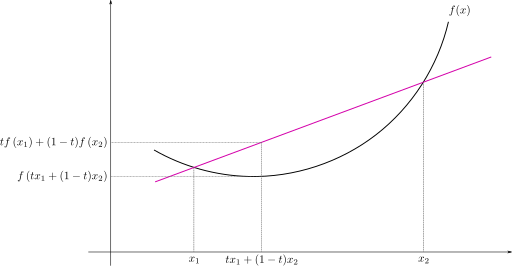
\includegraphics{convex.png}
\caption{convex}
\end{figure}

    Convex functions play an important role in many areas of mathematics.
They are especially important in the study of optimization problems
where they are distinguished by a number of convenient properties. For
instance, a (strictly) convex function on an open set has no more than
one minimum. Even in infinite-dimensioinal space, under suitable
additional hypotheses, convex functions continue to satisfy such
properties.

    \begin{figure}
\centering
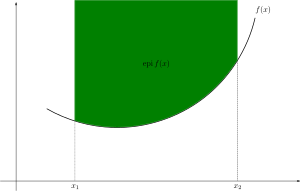
\includegraphics{convex-set.png}
\caption{convex set}
\end{figure}

    A function (in black) is convex if and only if the region above its
graph (in green) is a \textbf{convex set}. A convex set is a collection
of points such that, for each pair of points in the collection, the
entire line segment joining these two points is also in the collection.

    \hypertarget{concave}{%
\section{Concave}\label{concave}}

    A set that is not convex is a called a \emph{non-convex set}. A polygon
that is not a convex polygon is sometimes called a concave polygon, and
some sources more generally use the term \emph{concave set} to mean a
non-convex set, but most authorities prohibit this usage.

The complement of a convex set, such as the epigraph of a concave
function, is sometimes called a \emph{reverse convex set}, expecially in
the context of mathematical optimization.

    \hypertarget{single-variable-convexityconcavity-test}{%
\section{Single variable convexity/concavity
test}\label{single-variable-convexityconcavity-test}}

    Let \(f\) be any single variable function. We can test if \(f\) is
concave/convex by finding the second derivative of \(f\), and testing
the following three cases:

\begin{itemize}
\tightlist
\item
  \(f''(x) > 0 \rightarrow f\) is convex at \(x\).
\item
  \(f''(x) < 0 \rightarrow f\) is concave at \(x\).
\item
  \(f''(x) = 0 \rightarrow f\) has an inflection point at \(x\).
\end{itemize}

The inflection point determines when the function convexity/concavity of
\(f\) changes.

\hypertarget{example}{%
\subsection{Example}\label{example}}

Let \(f(x)=5x^3 + 4x^2 + 6x\). If we differentiate \(f\), we get
\(f'(x)=15x^2+8x+6\). Differentiating again, for the second derivative,
we get \(f''(x)=30x+8\). If we plot \(f(x)\) and \(f''(x)\), we get:

    \begin{Verbatim}[commandchars=\\\{\}]
{\color{incolor}In [{\color{incolor}5}]:} \PY{n}{X} \PY{o}{=} \PY{n}{np}\PY{o}{.}\PY{n}{linspace}\PY{p}{(}\PY{o}{\PYZhy{}}\PY{l+m+mi}{10}\PY{p}{,} \PY{l+m+mi}{10}\PY{p}{,} \PY{l+m+mi}{40}\PY{p}{)}                           \PY{c+c1}{\PYZsh{} x}
        \PY{n}{Y1} \PY{o}{=} \PY{p}{[}\PY{p}{(}\PY{k}{lambda} \PY{n}{x}\PY{p}{:} \PY{l+m+mi}{5}\PY{o}{*}\PY{n}{x}\PY{o}{*}\PY{o}{*}\PY{l+m+mi}{3} \PY{o}{+} \PY{l+m+mi}{4}\PY{o}{*}\PY{n}{x}\PY{o}{*}\PY{o}{*}\PY{l+m+mi}{2} \PY{o}{+} \PY{l+m+mi}{6}\PY{o}{*}\PY{n}{x}\PY{p}{)}\PY{p}{(}\PY{n}{x}\PY{p}{)} \PY{k}{for} \PY{n}{x} \PY{o+ow}{in} \PY{n}{X}\PY{p}{]} \PY{c+c1}{\PYZsh{} f(x)}
        \PY{n}{Y2} \PY{o}{=} \PY{p}{[}\PY{p}{(}\PY{k}{lambda} \PY{n}{x}\PY{p}{:} \PY{l+m+mi}{30}\PY{o}{*}\PY{n}{x} \PY{o}{+} \PY{l+m+mi}{8}\PY{p}{)}\PY{p}{(}\PY{n}{x}\PY{p}{)} \PY{k}{for} \PY{n}{x} \PY{o+ow}{in} \PY{n}{X}\PY{p}{]}              \PY{c+c1}{\PYZsh{} f\PYZsq{}\PYZsq{}(x)}
        \PY{n}{plot}\PY{p}{(}\PY{n}{X}\PY{p}{,}\PY{n}{Y1}\PY{p}{,}\PY{n}{c}\PY{o}{=}\PY{l+s+s1}{\PYZsq{}}\PY{l+s+s1}{b}\PY{l+s+s1}{\PYZsq{}}\PY{p}{,}\PY{n}{lw}\PY{o}{=}\PY{l+m+mi}{2}\PY{p}{)}
        \PY{n}{plot}\PY{p}{(}\PY{n}{X}\PY{p}{,}\PY{n}{Y2}\PY{p}{,}\PY{n}{c}\PY{o}{=}\PY{l+s+s1}{\PYZsq{}}\PY{l+s+s1}{r}\PY{l+s+s1}{\PYZsq{}}\PY{p}{,}\PY{n}{lw}\PY{o}{=}\PY{l+m+mi}{2}\PY{p}{,}\PY{n}{ls}\PY{o}{=}\PY{l+s+s1}{\PYZsq{}}\PY{l+s+s1}{dashed}\PY{l+s+s1}{\PYZsq{}}\PY{p}{)}
        \PY{n}{grid}\PY{p}{(}\PY{p}{)}\PY{p}{;}\PY{n}{xlabel}\PY{p}{(}\PY{l+s+s1}{\PYZsq{}}\PY{l+s+s1}{\PYZdl{}x\PYZdl{}}\PY{l+s+s1}{\PYZsq{}}\PY{p}{)}\PY{p}{;}\PY{n}{ylabel}\PY{p}{(}\PY{l+s+s1}{\PYZsq{}}\PY{l+s+s1}{\PYZdl{}f(x)\PYZdl{} and \PYZdl{}f}\PY{l+s+se}{\PYZbs{}\PYZsq{}}\PY{l+s+se}{\PYZbs{}\PYZsq{}}\PY{l+s+s1}{(x)\PYZdl{}}\PY{l+s+s1}{\PYZsq{}}\PY{p}{)}
        \PY{n}{title}\PY{p}{(}\PY{l+s+s1}{\PYZsq{}}\PY{l+s+s1}{Graph of \PYZdl{}f(x)\PYZdl{} and \PYZdl{}f}\PY{l+s+se}{\PYZbs{}\PYZsq{}}\PY{l+s+se}{\PYZbs{}\PYZsq{}}\PY{l+s+s1}{(x)\PYZdl{}}\PY{l+s+s1}{\PYZsq{}}\PY{p}{)}\PY{p}{;}
\end{Verbatim}


    \begin{center}
    \adjustimage{max size={0.9\linewidth}{0.9\paperheight}}{output_13_0.png}
    \end{center}
    { \hspace*{\fill} \\}
    
    We know the inflection point is where \(f''(x)=0\), therefore
\(30x+8=0\), which means that the inflection point is at
\(x=-\frac{8}{30}\).

Now we will test if the second derivative is positive/negative on each
side of the inflection point:

\begin{itemize}
\tightlist
\item
  \(f''(-5) = -142 \rightarrow f\) is concave at \(x=-5\).
\item
  \(f''(5) = 156 \rightarrow f\) is convex at \(x=5\).
\end{itemize}

Because we know the inflection point, we now know that \(f\) is convex
on the interval \(\left[-\frac{8}{30}, \rightarrow\right>\). In a
similar way, we also know that \(f\) is concave on the interval
\(\left<\leftarrow, -\frac{8}{30}\right]\).

    \hypertarget{two-variable-convexityconcavity-test}{%
\section{Two variable convexity/concavity
test}\label{two-variable-convexityconcavity-test}}

    We can also test for convexity/concavity for two variable functions. If
we look at an example function \(f(x,y)=x^2+xy+y^2\), we can clearly see
that it is strictly convex.

    \begin{Verbatim}[commandchars=\\\{\}]
{\color{incolor}In [{\color{incolor}6}]:} \PY{k+kn}{from} \PY{n+nn}{mpl\PYZus{}toolkits}\PY{n+nn}{.}\PY{n+nn}{mplot3d} \PY{k}{import} \PY{n}{Axes3D}
        \PY{n}{fig} \PY{o}{=} \PY{n}{plt}\PY{o}{.}\PY{n}{figure}\PY{p}{(}\PY{n}{figsize}\PY{o}{=}\PY{p}{(}\PY{l+m+mi}{14}\PY{p}{,}\PY{l+m+mi}{10}\PY{p}{)}\PY{p}{)}
        \PY{n}{ax} \PY{o}{=} \PY{n}{fig}\PY{o}{.}\PY{n}{add\PYZus{}subplot}\PY{p}{(}\PY{l+m+mi}{111}\PY{p}{,} \PY{n}{projection}\PY{o}{=}\PY{l+s+s1}{\PYZsq{}}\PY{l+s+s1}{3d}\PY{l+s+s1}{\PYZsq{}}\PY{p}{)}
        \PY{n}{xs} \PY{o}{=} \PY{n}{ys} \PY{o}{=} \PY{n}{np}\PY{o}{.}\PY{n}{arange}\PY{p}{(}\PY{o}{\PYZhy{}}\PY{l+m+mi}{5}\PY{p}{,} \PY{l+m+mi}{5}\PY{p}{,} \PY{o}{.}\PY{l+m+mi}{05}\PY{p}{)}
        \PY{n}{X}\PY{p}{,} \PY{n}{Y} \PY{o}{=} \PY{n}{np}\PY{o}{.}\PY{n}{meshgrid}\PY{p}{(}\PY{n}{xs}\PY{p}{,} \PY{n}{ys}\PY{p}{)}
        \PY{n}{zs} \PY{o}{=} \PY{n}{np}\PY{o}{.}\PY{n}{array}\PY{p}{(}\PY{p}{[}\PY{p}{(}\PY{k}{lambda} \PY{n}{x}\PY{p}{,} \PY{n}{y}\PY{p}{:} \PY{n}{x}\PY{o}{*}\PY{o}{*}\PY{l+m+mi}{2} \PY{o}{+} \PY{n}{x}\PY{o}{*}\PY{n}{y} \PY{o}{+} \PY{n}{y}\PY{o}{*}\PY{o}{*}\PY{l+m+mi}{2}\PY{p}{)}\PY{p}{(}\PY{n}{x}\PY{p}{,} \PY{n}{y}\PY{p}{)} \PY{k}{for} \PY{n}{x}\PY{p}{,} \PY{n}{y} \PY{o+ow}{in} \PY{n+nb}{zip}\PY{p}{(}\PY{n}{np}\PY{o}{.}\PY{n}{ravel}\PY{p}{(}\PY{n}{X}\PY{p}{)}\PY{p}{,} \PY{n}{np}\PY{o}{.}\PY{n}{ravel}\PY{p}{(}\PY{n}{Y}\PY{p}{)}\PY{p}{)}\PY{p}{]}\PY{p}{)}
        \PY{n}{Z} \PY{o}{=} \PY{n}{zs}\PY{o}{.}\PY{n}{reshape}\PY{p}{(}\PY{n}{X}\PY{o}{.}\PY{n}{shape}\PY{p}{)}
        \PY{n}{surf} \PY{o}{=} \PY{n}{ax}\PY{o}{.}\PY{n}{plot\PYZus{}surface}\PY{p}{(}\PY{n}{X}\PY{p}{,} \PY{n}{Y}\PY{p}{,} \PY{n}{Z}\PY{p}{,} \PY{n}{cmap}\PY{o}{=}\PY{n}{cm}\PY{o}{.}\PY{n}{jet}\PY{p}{)}
        \PY{n}{fig}\PY{o}{.}\PY{n}{colorbar}\PY{p}{(}\PY{n}{surf}\PY{p}{,} \PY{n}{shrink}\PY{o}{=}\PY{l+m+mf}{0.5}\PY{p}{,} \PY{n}{aspect}\PY{o}{=}\PY{l+m+mi}{5}\PY{p}{)}   
        \PY{n}{xlabel}\PY{p}{(}\PY{l+s+s1}{\PYZsq{}}\PY{l+s+s1}{X}\PY{l+s+s1}{\PYZsq{}}\PY{p}{)}\PY{p}{;}\PY{n}{ylabel}\PY{p}{(}\PY{l+s+s1}{\PYZsq{}}\PY{l+s+s1}{Y}\PY{l+s+s1}{\PYZsq{}}\PY{p}{)}\PY{p}{;}\PY{n}{ax}\PY{o}{.}\PY{n}{set\PYZus{}zlabel}\PY{p}{(}\PY{l+s+s1}{\PYZsq{}}\PY{l+s+s1}{\PYZdl{}f(x,y)\PYZdl{}}\PY{l+s+s1}{\PYZsq{}}\PY{p}{)}
        \PY{n}{title}\PY{p}{(}\PY{l+s+s1}{\PYZsq{}}\PY{l+s+s1}{Surface plot of \PYZdl{}f(x,y)=x\PYZca{}2+xy+y\PYZca{}2\PYZdl{}}\PY{l+s+s1}{\PYZsq{}}\PY{p}{)}\PY{p}{;}
\end{Verbatim}


    \begin{center}
    \adjustimage{max size={0.9\linewidth}{0.9\paperheight}}{output_17_0.png}
    \end{center}
    { \hspace*{\fill} \\}
    
    \hypertarget{method-for-functions-of-two-variables}{%
\subsection{Method for functions of two
variables}\label{method-for-functions-of-two-variables}}

    To determine if \(f(x,y)\) is concave or convex, we need to find the
following four quantities:

\begin{itemize}
\tightlist
\item
  \(\dfrac{\partial^2 f(x,y)}{\partial x^2}\) : The second partial
  derivative of \(f(x,y)\) with respect to \(x\).
\item
  \(\dfrac{\partial^2 f(x,y)}{\partial y^2}\) : The second partial
  derivative of \(f(x,y)\) with respect to \(y\).
\item
  \(\dfrac{\partial^2 f(x,y)}{\partial x \partial y}\) : The first
  partial with respect to \(x\), and the second partial with respect to
  \(y\).
\item
  \(\dfrac{\partial^2 f(x,y)}{\partial y \partial x}\) : The first
  partial with respect to \(y\), and the second partial with respect to
  \(x\).
\end{itemize}

    It is important to note that if we first take the partial with respect
to \(x\) and then with respect to \(y\), we will get the same as if we
first take it with respect to \(y\) and the with respect to \(x\). This
means that \(\dfrac{\partial^2 f(x,y)}{\partial x \partial y}\) is the
same as \(\dfrac{\partial^2 f(x,y)}{\partial y \partial x}\). Therefore
it is sufficient to find one of them, and squaring them to get
\(\left[\dfrac{\partial^2 f(x,y)}{\partial x \partial y}\right]^2\).

After we have found the quantities, we can compare them in the following
table to see if \(f(x,y)\) is convex/concave, or none at all:

    \begin{longtable}[]{@{}lllll@{}}
\toprule
\begin{minipage}[b]{0.17\columnwidth}\raggedright
Quantity\strut
\end{minipage} & \begin{minipage}[b]{0.17\columnwidth}\raggedright
Convex\strut
\end{minipage} & \begin{minipage}[b]{0.17\columnwidth}\raggedright
Strictly convex\strut
\end{minipage} & \begin{minipage}[b]{0.17\columnwidth}\raggedright
Concave\strut
\end{minipage} & \begin{minipage}[b]{0.17\columnwidth}\raggedright
Strictly concave\strut
\end{minipage}\tabularnewline
\midrule
\endhead
\begin{minipage}[t]{0.17\columnwidth}\raggedright
\(\dfrac{\partial^2 f(x,y)}{\partial x^2} \cdot \dfrac{\partial^2 f(x,y)}{\partial y^2} - \left[ \dfrac{\partial^2 f(x,y)}{\partial x \partial y} \right]^2\)\strut
\end{minipage} & \begin{minipage}[t]{0.17\columnwidth}\raggedright
\(\geq 0\)\strut
\end{minipage} & \begin{minipage}[t]{0.17\columnwidth}\raggedright
\(>0\)\strut
\end{minipage} & \begin{minipage}[t]{0.17\columnwidth}\raggedright
\(\geq 0\)\strut
\end{minipage} & \begin{minipage}[t]{0.17\columnwidth}\raggedright
\(> 0\)\strut
\end{minipage}\tabularnewline
\begin{minipage}[t]{0.17\columnwidth}\raggedright
\(\dfrac{\partial^2 f(x,y)}{\partial x^2}\)\strut
\end{minipage} & \begin{minipage}[t]{0.17\columnwidth}\raggedright
\(\geq 0\)\strut
\end{minipage} & \begin{minipage}[t]{0.17\columnwidth}\raggedright
\(>0\)\strut
\end{minipage} & \begin{minipage}[t]{0.17\columnwidth}\raggedright
\(\leq 0\)\strut
\end{minipage} & \begin{minipage}[t]{0.17\columnwidth}\raggedright
\(< 0\)\strut
\end{minipage}\tabularnewline
\begin{minipage}[t]{0.17\columnwidth}\raggedright
\(\dfrac{\partial^2 f(x,y)}{\partial y^2}\)\strut
\end{minipage} & \begin{minipage}[t]{0.17\columnwidth}\raggedright
\(\geq 0\)\strut
\end{minipage} & \begin{minipage}[t]{0.17\columnwidth}\raggedright
\(>0\)\strut
\end{minipage} & \begin{minipage}[t]{0.17\columnwidth}\raggedright
\(\leq 0\)\strut
\end{minipage} & \begin{minipage}[t]{0.17\columnwidth}\raggedright
\(< 0\)\strut
\end{minipage}\tabularnewline
\bottomrule
\end{longtable}

    A quick way to determine if a function is convex or concave, is by
finding the quantities in the following matrix:

\[ M = \begin{bmatrix} \dfrac{\partial^2 f(x,y)}{\partial x^2} & \dfrac{\partial^2 f(x,y)}{\partial x \partial y} \\ \dfrac{\partial^2 f(x,y)}{\partial y^2} & \dfrac{\partial^2 f(x,y)}{\partial y \partial x}  \end{bmatrix} \]

    If \(f(x,y)\) is convex/concave, this means that
\(\textrm{det}(M) \geq 0\). If we remember that
\(\text{det}(M) = \dfrac{1}{ad-bc}\), we can see that the
\(\textrm{det}(M)\) becomes:

\[ \dfrac{1}{\dfrac{\partial^2 f(x,y)}{\partial x^2} \cdot \dfrac{\partial^2 f(x,y)}{\partial y^2} - \dfrac{\partial^2 f(x,y)}{\partial x \partial y} \cdot \dfrac{\partial^2 f(x,y)}{\partial y \partial x} } \geq 0 \]

    But if we recall that
\(\dfrac{\partial^2 f(x,y)}{\partial x \partial y}\) is the same as
\(\dfrac{\partial^2 f(x,y)}{\partial y \partial x}\), we can rewrite it
as:

\[ \dfrac{1}{\dfrac{\partial^2 f(x,y)}{\partial x^2} \cdot \dfrac{\partial^2 f(x,y)}{\partial y^2} - \left[\dfrac{\partial^2 f(x,y)}{\partial x \partial y}\right]^2  } \geq 0.\]

But because we only want to determine if the result is zero or positive,
we can conclude that

\[ \dfrac{\partial^2 f(x,y)}{\partial x^2} \cdot \dfrac{\partial^2 f(x,y)}{\partial y^2} - \left[\dfrac{\partial^2 f(x,y)}{\partial x \partial y}\right]^2 \geq 0,\]

which is the quantity in the table.

    \hypertarget{example}{%
\subsection{Example}\label{example}}

    Let \(f(x,y)=x^2+xy+y^2\). We first determine the four quantities:

\begin{itemize}
\tightlist
\item
  \(\dfrac{\partial^2 f(x,y)}{\partial x^2} = 2\).
\item
  \(\dfrac{\partial^2 f(x,y)}{\partial y^2} = 2\).
\item
  \(\dfrac{\partial^2 f(x,y)}{\partial x \partial y} = 1\).
\item
  \(\dfrac{\partial^2 f(x,y)}{\partial y \partial x} = 1\).
\end{itemize}

If we let \(M=\begin{bmatrix} 2 && 1 \\ 1 && 2 \end{bmatrix}\) we find
that
\(\textrm{det}(M)=\dfrac{1}{2\cdot2-1\cdot1} = \dfrac{1}{4-1} = \dfrac{1}{3}\).
This means that the function is either convex or concave.

If we look at the table we can see that
\(\dfrac{\partial^2 f(x,y)}{\partial x^2} > 0\) and
\(\dfrac{\partial^2 f(x,y)}{\partial y^2} > 0\). This means that
\(f(x,y)\) is a strictly convex function.

    \hypertarget{references}{%
\section{References}\label{references}}

    \begin{enumerate}
\def\labelenumi{\arabic{enumi}.}
\tightlist
\item
  https://en.wikipedia.org/wiki/Convex\_set
\item
  https://en.wikipedia.org/wiki/Convex\_function
\item
  Introduction to Operations Research, Hillier/Lieberman, chapter 13.
\end{enumerate}


    % Add a bibliography block to the postdoc
    
    
    
    \end{document}
